\section{Auswertung}
\label{sec:Auswertung}

\subsection{Fourier-Analyse}
\label{sec:Auswertung_Analyse}

Am Funktionsgenerator wurden folgende Spannungen eingestellt, für die das Oszilloskop die Fourier-Transformation durchführt (siehe Tabelle \ref{tab:Generator}).
\begin{table}
  \centering
  \caption{Konfiguration des Funktionsgenerators.}
  \label{tab:Generator}
  \begin{tabular}{c c c}
    \toprule
    & Frequenz in kHz & Amplitude in V \\
    \midrule
    Rechteckspannung & 120 & 10 \\
    Sägezahnspannung & 100 & 10 \\
    Dreieckspannung & 100 & 10 \\
    \bottomrule
  \end{tabular}
\end{table}
Um die gemessenen Amplituden vernünftig mit den berechneten Fourier-Koeffizienten vergleichen zu können, sollen die Messdaten doppellogarithmisch dargestellt werden.
Das bringt den Vorteil, dass die Potenzfunktionen zu Geraden werden, deren Steigung dem Exponenten entspricht.
\begin{align*}
   y &= a \cdot x^n \\
   \intertext{Wird der natürliche Logarithmus angewendet, folgt:}
   \lg(y) &= \lg(a) + n \cdot \lg(x) \\
   Y &= n \cdot X + C \\
   \text{mit} \lg(y) &= Y \quad \lg(x) = x \quad \lg(a) = C
\end{align*}
Vor der Anwendung des Logarithmus werden die Amplituden auf die Amplitude der ersten Oberwelle geeicht.
Anschließend wird über lineare Regression ein Fit für die Messdaten erstellt (siehe Abbildung \ref{fig:plot1}, \ref{fig:plot2} und \ref{fig:plot3}).
Die Steigung dieser Ausgleichsgeraden kann dann mit der Potenz mit der die Amplituden abfallen verglichen werden.
Die Abweichung von Theorie und Messung wird mit folgender Formel bestimmt.
\begin{equation}
  \increment m = \left \lvert \frac{m_{\text{Theorie}} - m_{\text{Messung}}}{m_{\text{Theorie}}} \right \rvert
\end{equation}
Für die drei verschiedenen Spannungen ergaben sich folgende Ergebnisse:
\begin{align*}
  \intertext{Rechteckspannung}
  m_{\text{Messung}} &= -0,9977 \pm 0,0141 & m_{\text{Theorie}} &= -1 & \increment m &= 0,23 \%
  \intertext{Sägezahnspannung}
  m_{\text{Messung}} &= -1,0085 \pm 0,0286 & m_{\text{Theorie}} &= -1 & \increment m &= 0,85 \%
  \intertext{Dreieckspannung}
  m_{\text{Messung}} &= -2,0126 \pm 0,0325 & m_{\text{Theorie}} &= -2 & \increment m &= 0,63 \%
\end{align*}
\begin{figure}
  \centering
  \includegraphics{plot1.pdf}
  \caption{Amplituden der Rechteckspannung.}
  \label{fig:plot1}
\end{figure}
\begin{figure}
  \centering
  \includegraphics{plot2.pdf}
  \caption{Amplituden der Sägezahnspannung.}
  \label{fig:plot2}
\end{figure}
\begin{figure}
  \centering
  \includegraphics{plot3.pdf}
  \caption{Amplituden der Dreieckspannung.}
  \label{fig:plot3}
\end{figure}

\FloatBarrier

\subsection{Fourier-Synthese}
\label{sec:Auswertung_Synthese}

Die zuvor berechneten Koeffizienten (siehe \ref{sec:Koeffizienten}) für die ersten 9 Oberwellen werden am Signalgenerator eingestellt.
Nachdem die Phasen am Signalgenerator feinjustiert wurden, ergaben sich auf dem Oszilloskop die Spannungsverläufe, die in den folgenden Abbildungen zu sehen sind.

\subsubsection{Sythese der Rechteckspannung}
Die Spannungsfunktion hat eine Amplitude 1,45 Volt und eine Frequenz von 440 Hertz (Abbildung \ref{fig:abb4}).
\begin{figure}
  \centering
  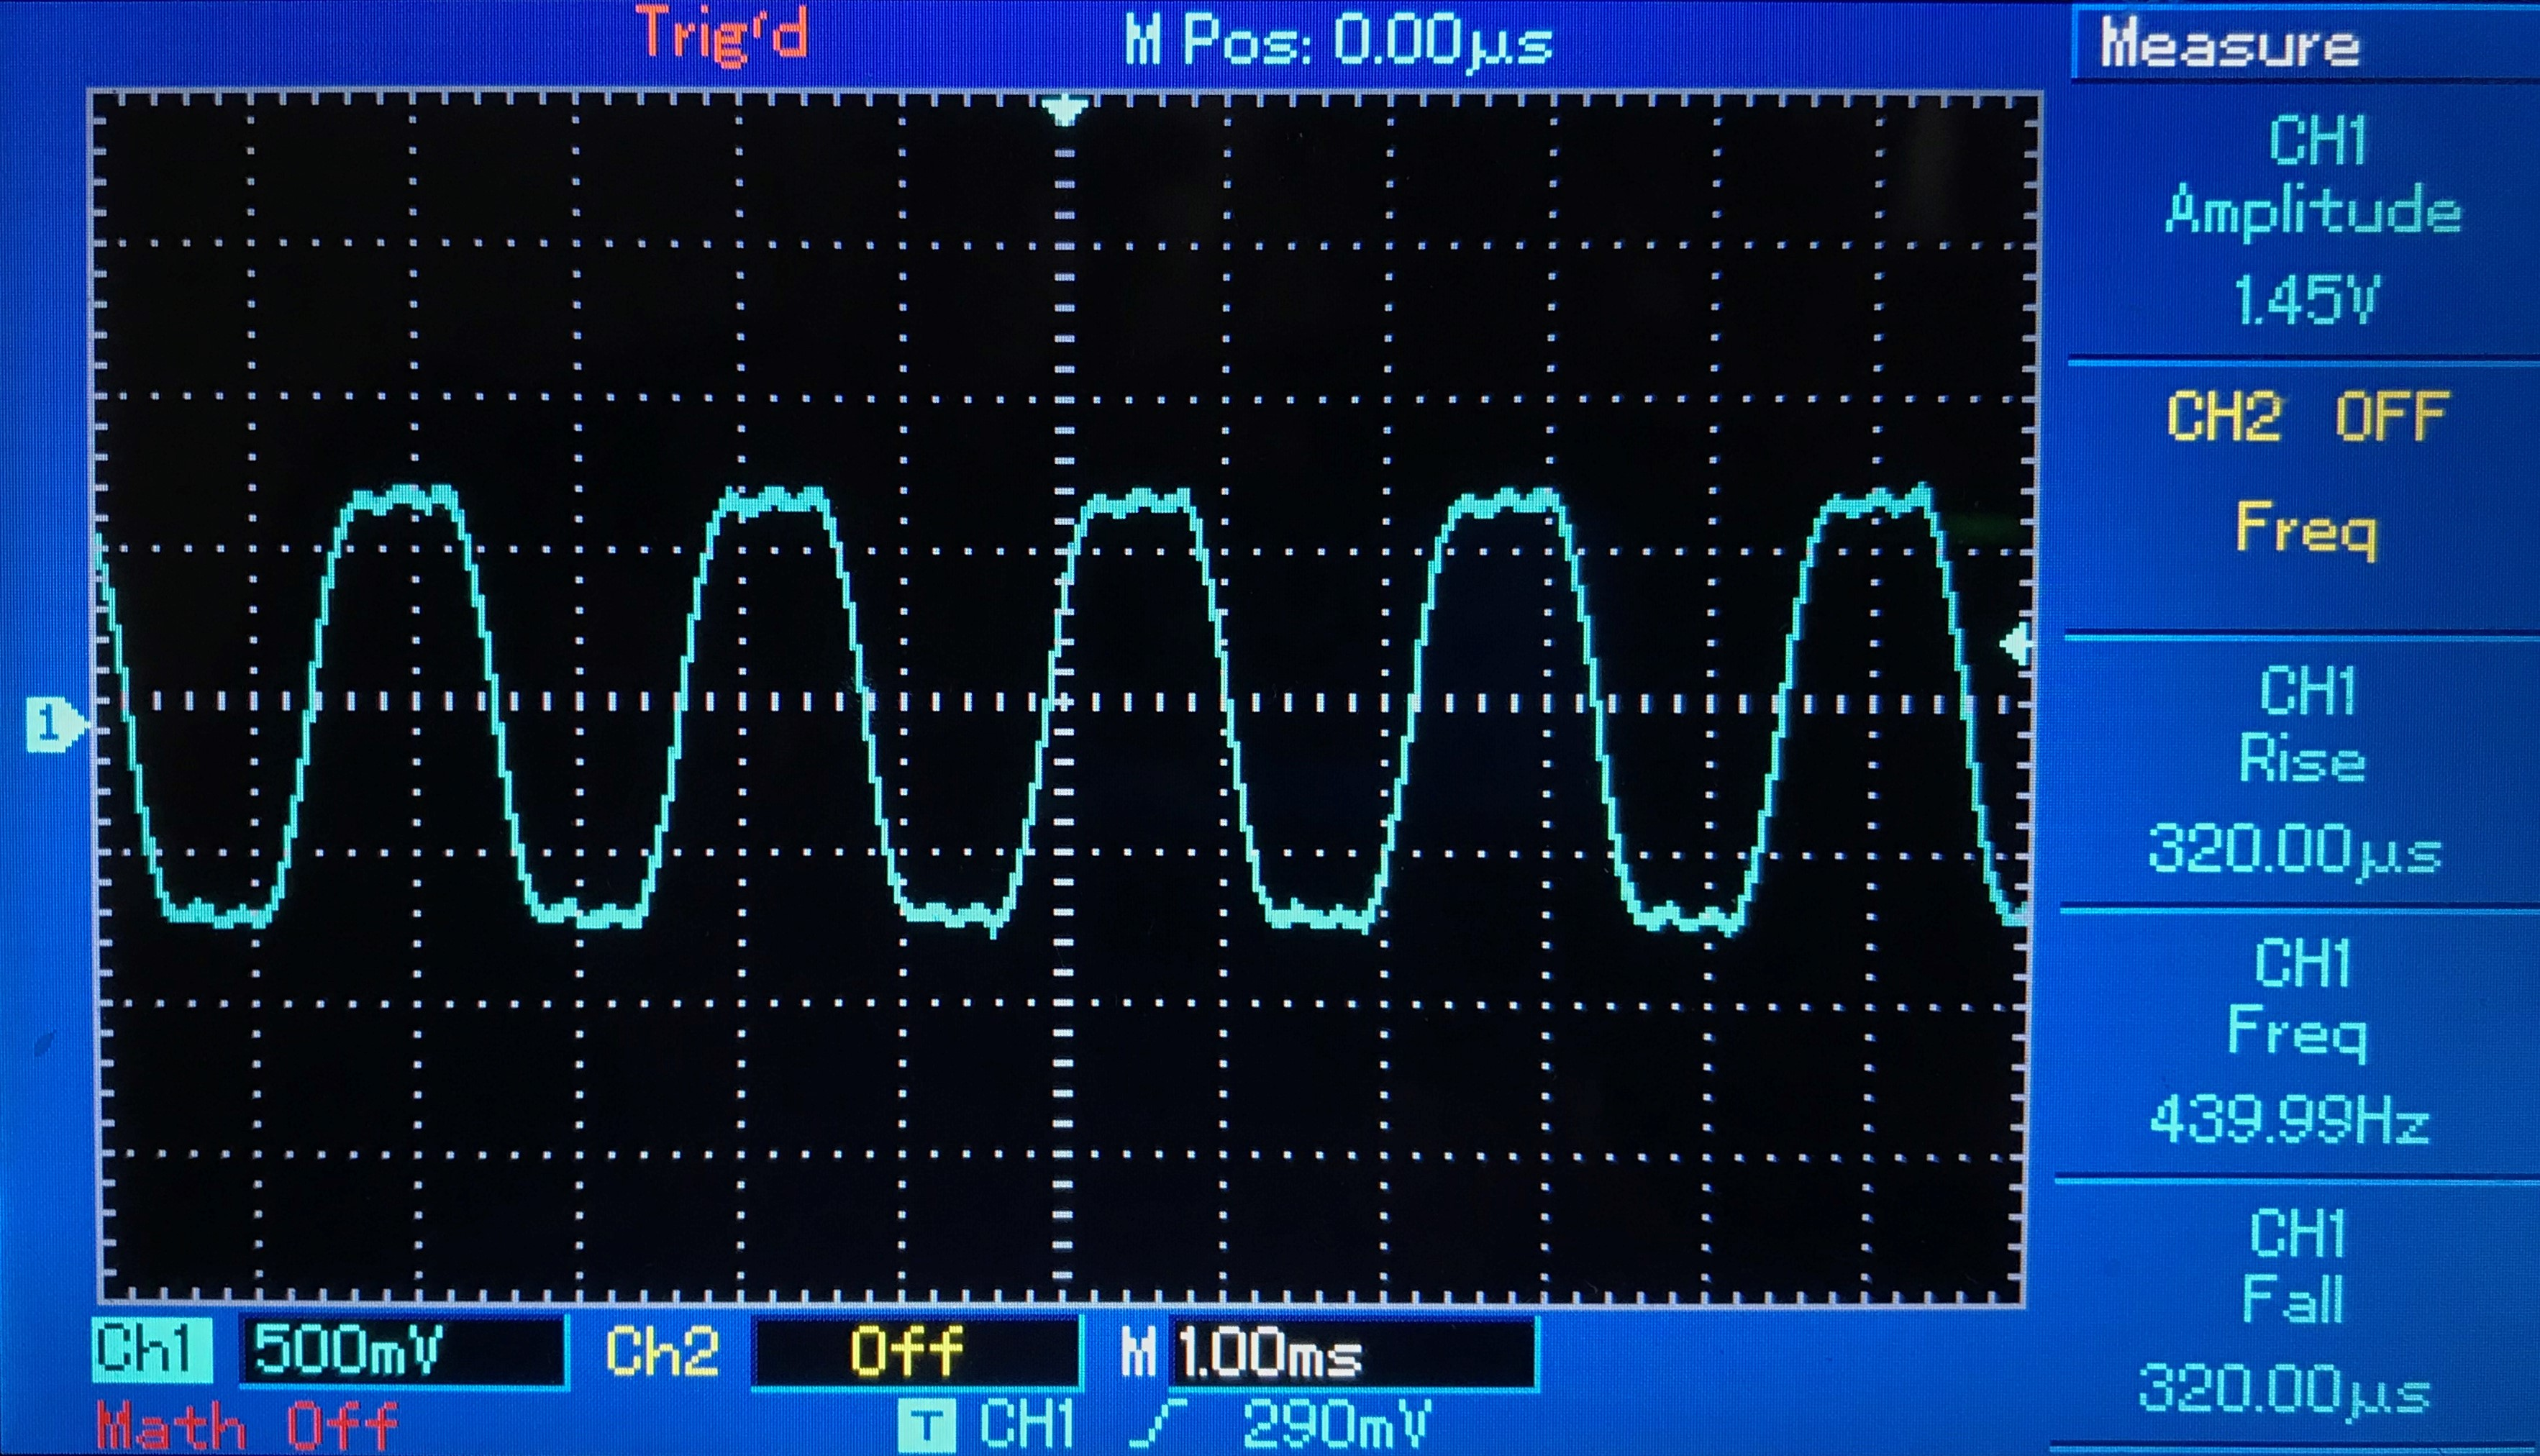
\includegraphics[width=\textwidth]{abb4.jpg}
  \caption{synthetisierte Rechteckspannung.}
  \label{fig:abb4}
\end{figure}
\subsubsection{Synthese der Sägezahnspannung}
Die Spannungsfunktion hat eine Amplitude 2,14 Volt und eine Frequenz von 440 Hertz (Abbildung \ref{fig:abb5}).
\begin{figure}
  \centering
  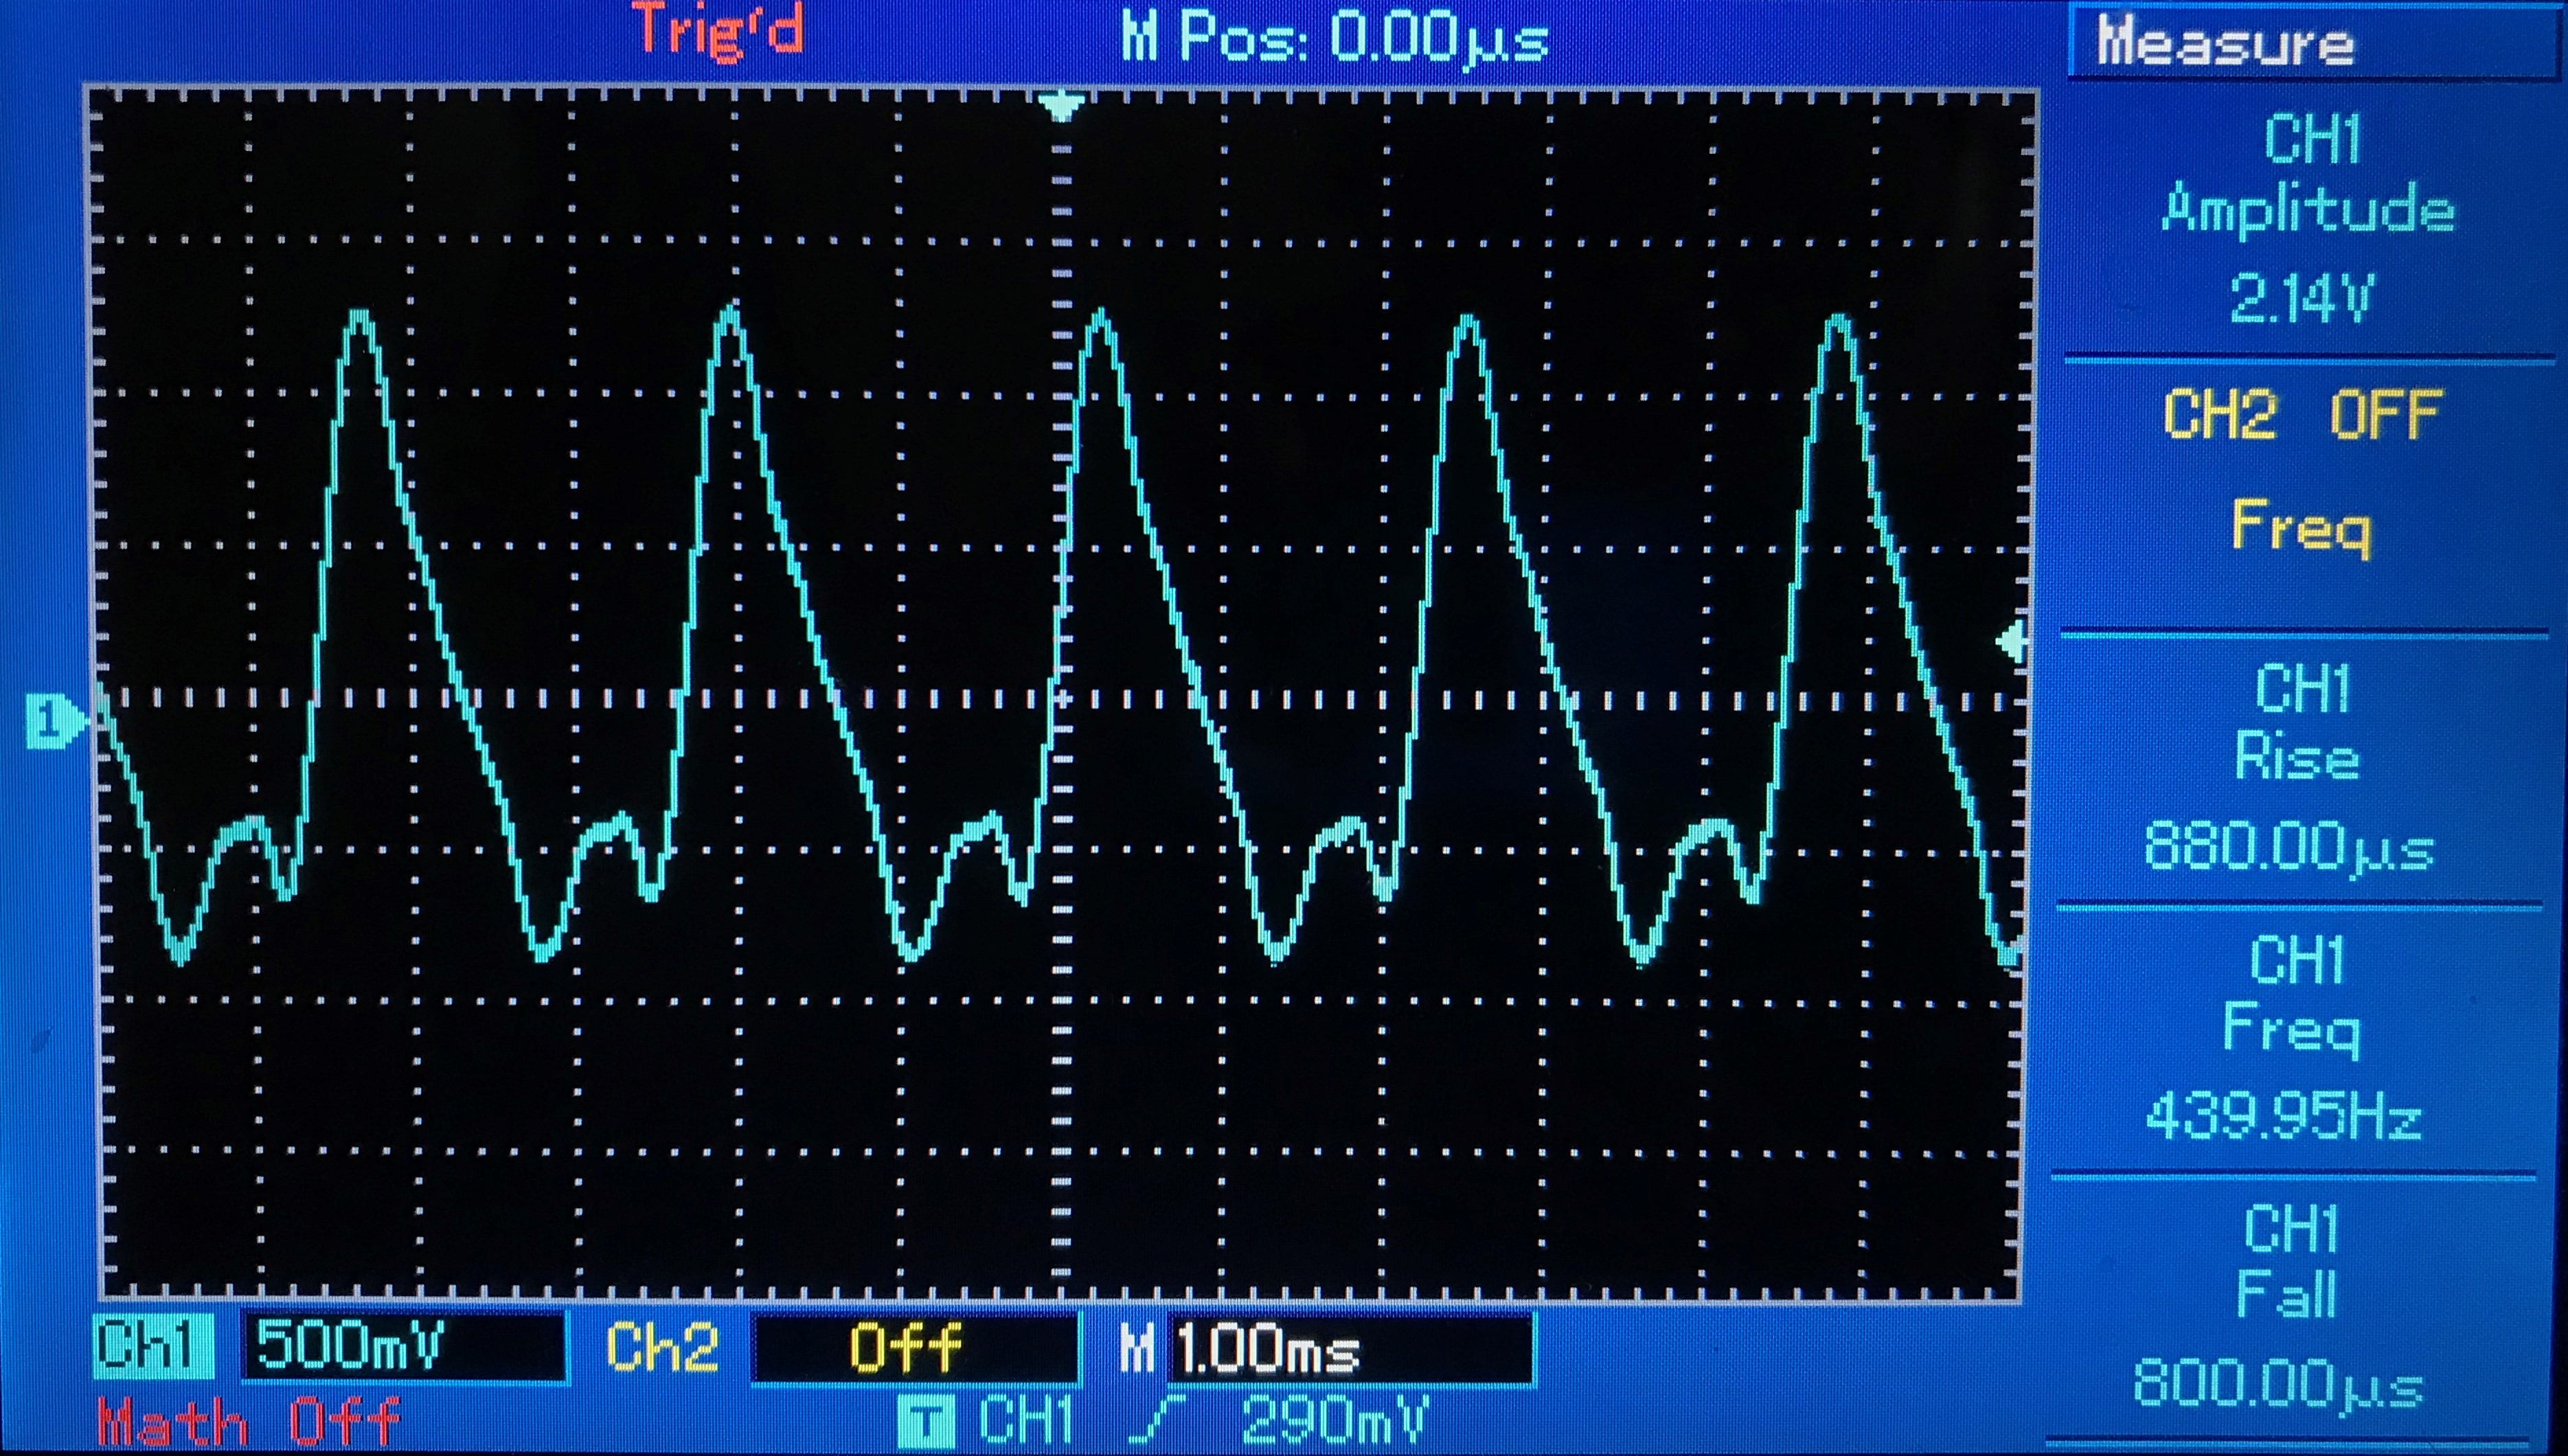
\includegraphics[width=\textwidth]{abb5.jpg}
  \caption{synthetisierte Sägezahnspannung.}
  \label{fig:abb5}
\end{figure}
\subsubsection{Synthese der Dreieckspannung}
Die Spannungsfunktion hat eine Amplitude 1,90 Volt und eine Frequenz von 440 Hertz (Abbildung \ref{fig:abb6}).
\begin{figure}
  \centering
  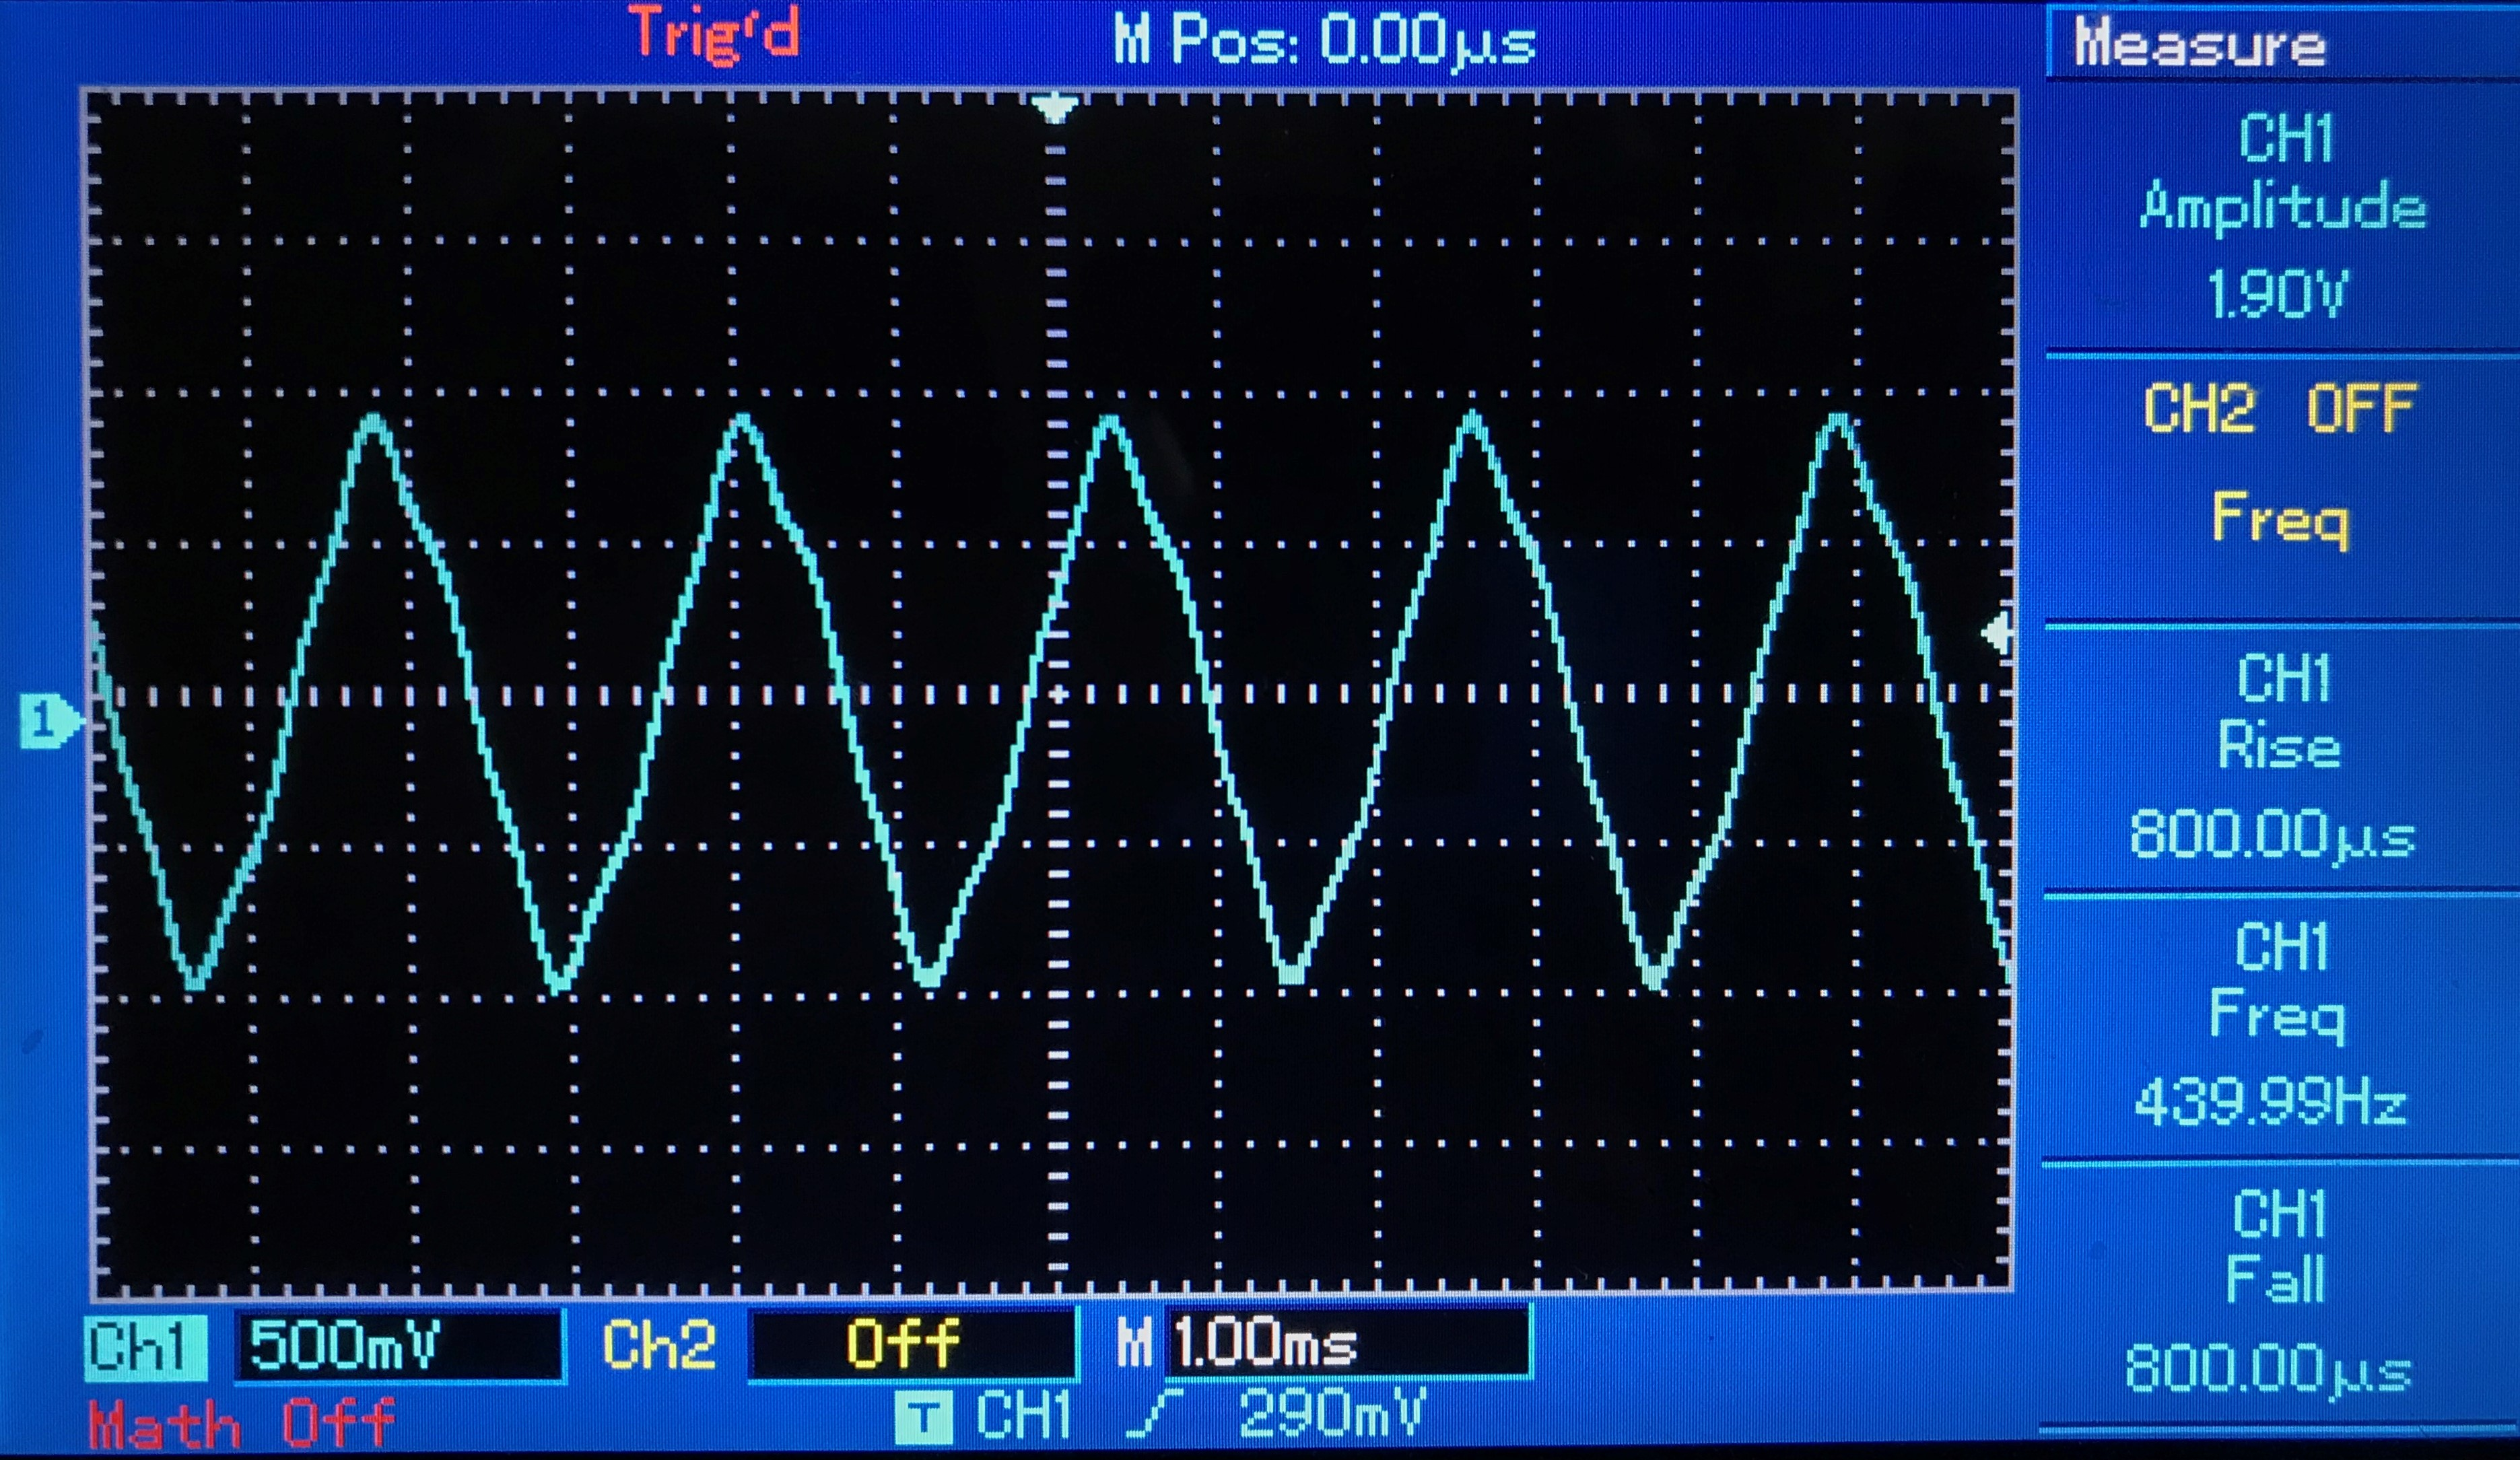
\includegraphics[width=\textwidth]{abb6.jpg}
  \caption{synthetisierte Dreieckspannung.}
  \label{fig:abb6}
\end{figure}
